\documentclass[11pt,twocolumn,a4paper]{article}

% ============================================================
%  FEDERATED KNAPSACK-ALLOCATED CASCADES
%  A Multi-Modal Architecture for Bounded-Receiver Inference
% ============================================================

\usepackage[utf8]{inputenc}
\usepackage[T1]{fontenc}
\usepackage{lmodern}
\usepackage[a4paper,margin=2.1cm,top=2.3cm,bottom=2.3cm,columnsep=0.6cm]{geometry}
\usepackage{amsmath,amssymb,amsthm,mathtools}
\usepackage{amsfonts,bm,stmaryrd,mathrsfs}
\usepackage{booktabs,array,multirow}
\usepackage{enumitem}
\usepackage{xcolor}
\usepackage[colorlinks=true,linkcolor=blue!50!black,citecolor=blue!50!black,urlcolor=blue!50!black]{hyperref}
\usepackage[round]{natbib}
\usepackage{microtype}
\usepackage{graphicx}
\usepackage{fancyhdr}
\usepackage{caption}
\usepackage{subcaption}
\usepackage{algorithm}
\usepackage{algpseudocode}
\usepackage{tikz}
\usetikzlibrary{arrows.meta,positioning,fit,calc,shapes.geometric}

% ---- theorem environments ----
\newtheorem{theorem}{Theorem}[section]
\newtheorem{lemma}[theorem]{Lemma}
\newtheorem{proposition}[theorem]{Proposition}
\newtheorem{corollary}[theorem]{Corollary}
\theoremstyle{definition}
\newtheorem{definition}[theorem]{Definition}
\newtheorem{axiom}[theorem]{Axiom}
\theoremstyle{remark}
\newtheorem{remark}[theorem]{Remark}
\newtheorem{example}[theorem]{Example}
\newtheorem{construction}[theorem]{Construction}

% ---- notation ----
\DeclareMathOperator*{\argmin}{arg\,min}
\DeclareMathOperator*{\argmax}{arg\,max}
\DeclareMathOperator{\diam}{diam}
\DeclareMathOperator{\dom}{dom}
\DeclareMathOperator{\img}{im}
\DeclareMathOperator{\Hom}{Hom}
\DeclareMathOperator{\id}{id}
\DeclareMathOperator{\eval}{eval}
\DeclareMathOperator{\dec}{dec}
\DeclareMathOperator{\KL}{KL}

\newcommand{\R}{\mathbb{R}}
\newcommand{\N}{\mathbb{N}}
\newcommand{\Z}{\mathbb{Z}}
\newcommand{\E}{\mathbb{E}}
\newcommand{\Prob}{\mathbb{P}}
\newcommand{\Cands}{\mathcal{X}}
\newcommand{\Action}{\mathcal{Y}}
\newcommand{\Knowl}{\mathcal{K}}
\newcommand{\Cell}{\mathcal{C}}
\newcommand{\Method}{\mathfrak{M}}
\newcommand{\Federation}{\mathfrak{F}}
\newcommand{\receiver}{\mathcal{R}}
\newcommand{\Sigmax}{\Sigma}
\newcommand{\Sscalar}{S}
\newcommand{\Sfloor}{S_{\flat}}
\newcommand{\hbarR}{\hbar_{\receiver}}
\newcommand{\catpow}{\kappa}
\newcommand{\disp}{\sigma}
\newcommand{\Know}{\mathrm{Know}}
\newcommand{\Hknow}{\mathfrak{H}}
\newcommand{\Compose}{\diamond}
\newcommand{\eps}{\varepsilon}

\pagestyle{fancy}
\fancyhf{}
\fancyhead[L]{\small\textit{Federated Knapsack-Allocated Cascades}}
\fancyhead[R]{\small\thepage}
\renewcommand{\headrulewidth}{0.4pt}

\title{\textbf{Federated Knapsack-Allocated Cascades:\\[3pt]
A Multi-Modal Architecture for Bounded-Receiver Inference\\[1pt]
with Provable Floor Reduction and Circular Coherence}}

\author{Kundai Farai Sachikonye\\
Technical University of Munich\\
\texttt{kundai.sachikonye@wzw.tum.de}}

\date{\today}

\begin{document}
\twocolumn[
  \begin{@twocolumnfalse}
    \maketitle
    \begin{abstract}
\noindent
We develop a complete mathematical theory and operational architecture for multi-model inference in which a finite federation of bounded models is composed under a knapsack-allocated cascade and validated by a circular cross-check graph. The architecture rests on six theorem clusters, each proved from first principles. (i)~\textbf{Floor Positivity}: every bounded inference system has a strictly positive irreducible error floor $\beta > 0$ on a normalised semantic-distance scale $[0,\Sigmax]$, attained as the supremum of unresolved alignment between its internal candidate set and the truth region. (ii)~\textbf{Methodological Composition}: an iterative refinement methodology with contraction $\catpow \in [0,1)$ and per-iteration dispersion $\disp$ has Banach-fixed-point floor $\disp\catpow/(1-\catpow)$ that cannot be reduced by repetition of the same methodology; composition of independent methodologies obeys a multiplicative catalytic law $\catpow(\gamma_1 \Compose \gamma_2) = 1 - (1-\catpow_1)(1-\catpow_2)$. (iii)~\textbf{Receiver Uncertainty Principle}: knowledge-space dispersion and action-space dispersion of any system are jointly bounded below by the product of its floor and the action tolerance, $\disp_K \cdot \disp_Y \geq \beta \tau$, a Heisenberg-type inequality with closed-form constant. (iv)~\textbf{Federation Inequality}: a federation of $n$ bounded systems with min-aggregating joint receiver attains aggregate floor $\Sfloor(\Federation) \leq \min_i \Sfloor(\receiver_i)$, with strict inequality whenever the systems are not mutually redundant; we give a closed-form expression for the marginal floor reduction obtained by adding each system. (v)~\textbf{Cascade Switching Theorem}: the optimal allocation of a finite inference budget across $k$ methodologies with floors $\beta_i$ and per-call costs $c_i$ is the value-density 0-1 knapsack on values $v_i = \log(\Sigmax/(\Sigmax - \beta_i))$, with the dual-density greedy admitting a $(1-1/e)$-approximation guarantee under the standard relaxation. (vi)~\textbf{Circular Validity}: linear (non-cyclic) justification fails for any bounded system because terminal nodes of the justification graph have no validator; a strongly-connected support graph of size $\geq 3$ is both necessary and sufficient for foundational coherence, formalised as a fixed-point existence theorem on the validator composition map. From these six clusters we synthesise the \emph{Federated Knapsack-Allocated Cascade} (FKAC) architecture, comprising a router (cascade switching), a parallel drafting layer (federation), a circular validator (three-way cross-check), and an integration layer with floor inheritance. We provide a complete operational specification of FKAC with end-to-end complexity analysis, prove an \emph{End-to-End Floor Theorem} bounding the architecture's effective floor below the floor of every constituent system, and instantiate the architecture on a representative inference task --- compilation of natural-language experiment specifications into procedural synthesis documents using a federation of open-weight language models. We report quantitative results showing the FKAC architecture reduces aggregate floor by a factor of 2.7--4.1 over best-single-model baselines and 1.4--1.9 over pairwise voting, with cascade allocation matching the knapsack optimum to within $5\%$ on calibrated benchmarks. The framework is presented as pure mathematics; every claim is proved, every algorithm has complexity bounds, every theorem is verified by a numerical experiment. Citations are restricted to standard literature; the development is self-contained.
\end{abstract}

\vspace{6pt}
\noindent\textbf{Keywords:} bounded inference, multi-model architecture, federation entropy, knapsack-allocated cascades, circular validation, methodological floor, multiplicative catalysts, action-cell coordination, ensemble inference, model routing.
\vspace{8pt}
  \end{@twocolumnfalse}
]

\tableofcontents

\vspace{6pt}
\hrule
\vspace{6pt}

% ============================================================
\part{Theoretical Foundations}
% ============================================================

\section{Introduction}
\label{sec:intro}

\subsection{The bounded-inference problem}

A long line of work in the foundations of computation, learning, and rational agency observes that any physically realised inference system---human, machine, or institutional---operates under bounded resources: bounded memory \citep{simon1956rational,simon1957models}, bounded sample size \citep{valiant1984theory,vapnik1998statistical,blumer1989learnability}, bounded representational capacity \citep{godel1931formal,turing1936computable}, bounded thermodynamic budget \citep{shannon1948mathematical,cover2006elements}. The consequences of boundedness are widely studied in isolation but rarely brought into a single calculus from which an operational architecture follows.

We are concerned in this paper with the following operational question. Given a finite collection of bounded inference systems, each with its own internal representation and irreducible error, and given a query whose ideal output lies in some target region of an outcome space, how should the systems be composed to produce an output whose error is provably smaller than any single system could achieve? Specifically, we want a composition rule for which (a) the joint error is bounded above by an explicit function of the constituents' floors, (b) the allocation of inference effort across constituents is optimal in a formally specified sense, and (c) the composition is foundationally coherent in the sense that its output is mutually validated and not merely chained.

The standard ensemble literature \citep{dietterich2000ensemble,breiman2001random,freund1997decision,wolpert1992stacked} provides bagging, boosting, stacking, and mixtures of experts \citep{jacobs1991adaptive,shazeer2017outrageously,fedus2022switch}, each with strong empirical track records and partial theoretical guarantees. Recent work on language-model ensembles \citep{wang2022self,du2023improving,jiang2023llm,wang2024mixture} extends these ideas to large pretrained models, with a focus on accuracy gains under fixed budget. Cost-aware routing approaches \citep{chen2023frugalgpt,sakota2024fly,lu2024merge,ong2024routellm,liu2024routerbench,aggarwal2024automix,naik2024diversity} treat the multi-model setting as an explicit optimisation problem: which model should answer which query, and in what order, subject to a budget. None of these works, however, prove a lower bound on attainable error across composition, identify the optimal allocation as a closed-form combinatorial-optimisation problem, or formalise the coherence property that distinguishes a foundationally validated composition from a chain of unchecked outputs.

\subsection{Contribution}

This paper develops a self-contained mathematical framework for composing bounded inference systems and proves four operational results that together specify a complete multi-model architecture, the \emph{Federated Knapsack-Allocated Cascade} (FKAC). The framework rests on a single primitive, the receiver-relative scalar functional $\Sscalar(\receiver, x; \Cell)$ measuring residual semantic distance between a system's processing of an input $x$ and an action-cell $\Cell$ (an equivalence class of acceptable outputs). From this primitive we prove:

\begin{itemize}[leftmargin=*,nosep]
\item \textbf{(Floor Positivity, Theorem~\ref{thm:floor})} Every bounded system $\receiver$ has irreducible floor $\Sfloor(\receiver) > 0$.
\item \textbf{(Methodological Floor, Theorem~\ref{thm:method-floor})} Every methodology has Banach-fixed-point floor $\disp\catpow/(1-\catpow)$ that cannot be reduced by repetition.
\item \textbf{(Catalytic Composition, Theorem~\ref{thm:catalytic})} Independent methodologies compose multiplicatively: $\catpow(\gamma_1 \Compose \gamma_2) = 1 - (1-\catpow_1)(1-\catpow_2)$.
\item \textbf{(Receiver Uncertainty Principle, Theorem~\ref{thm:uncertainty})} $\disp_K \cdot \disp_Y \geq \beta\tau$.
\item \textbf{(Federation Inequality, Theorem~\ref{thm:federation})} A federation of $n$ systems attains aggregate floor $\Sfloor(\Federation) \leq \min_i \Sfloor(\receiver_i)$, strict unless redundant.
\item \textbf{(Cascade Switching, Theorem~\ref{thm:knapsack})} Optimal budget allocation across $k$ methodologies is the 0-1 knapsack on values $v_i = \log(\Sigmax/(\Sigmax - \beta_i))$.
\item \textbf{(Circular Validity, Theorem~\ref{thm:circular})} Foundational coherence requires a strongly-connected validator graph of size $\geq 3$; linear justification fails by the floor theorem.
\item \textbf{(End-to-End Floor Bound, Theorem~\ref{thm:fkac})} The FKAC architecture attains effective floor strictly below the floor of every constituent system, with quantitative bound expressed in closed form.
\end{itemize}

The architecture is operational: every theorem corresponds to an algorithmic component, every component has complexity bound, every theorem is verified by a numerical experiment whose result is presented in the validation section.

\subsection{Position relative to existing approaches}

The framework subsumes several existing approaches as special or limiting cases:

\begin{itemize}[leftmargin=*,nosep]
\item \textbf{Single-model inference} is the $|\Federation| = 1$ case; the floor reduces to $\Sfloor(\receiver_1)$, which is strictly worse than $\Sfloor(\Federation)$ when $|\Federation| > 1$.
\item \textbf{Self-consistency} \citep{wang2022self} is the homogeneous-federation case with the same model run multiple times; the Methodological Floor theorem shows this cannot reduce error below $\disp\catpow/(1-\catpow)$ for the underlying model, formalising the empirical observation that self-consistency gains saturate quickly.
\item \textbf{Mixture-of-experts} \citep{jacobs1991adaptive,shazeer2017outrageously,fedus2022switch} is a parametric (single-trainable-gate) instance of the more general Federation construction; the FKAC architecture replaces the trainable gate with a knapsack-optimal closed-form router.
\item \textbf{Cost-aware cascade routing} \citep{chen2023frugalgpt,sakota2024fly,ong2024routellm} solves a special case of the Cascade Switching Theorem with $k = 2$ (cheap/expensive) and a learned router; we generalise to arbitrary $k$ with a closed-form optimum.
\item \textbf{Multi-agent debate} \citep{du2023improving,madaan2023self,wang2024mixture} is closely related to the Circular Validity step but lacks the formal lower bound on validator-graph size derived here.
\end{itemize}

\subsection{Independence}

The development is mathematically independent. Citations are restricted to standard references in real analysis \citep{rudin1987real}, measure theory \citep{halmos1950measure,kolmogorov1933foundations}, information theory \citep{shannon1948mathematical,cover2006elements,kullback1951information,kelly1956new}, statistical inference \citep{fisher1925theory,rao1945information}, fixed-point theory \citep{banach1922operations}, convex optimisation \citep{boyd2004convex,nesterov2018lectures}, combinatorial optimisation \citep{karp1972reducibility,dantzig1957discrete,bellman1957dynamic,kellerer2004knapsack,pisinger1997minimal,ibarra1975fast,garey1979computers}, PAC learning \citep{valiant1984theory,vapnik1998statistical,blumer1989learnability,shalev2014understanding}, the uncertainty principle \citep{heisenberg1927uber,robertson1929uncertainty}, classical ensemble learning \citep{dietterich2000ensemble,breiman2001random,freund1997decision,schapire1990strength,wolpert1992stacked}, mixture-of-experts and routing \citep{jacobs1991adaptive,shazeer2017outrageously,fedus2022switch}, foundational logic \citep{godel1931formal,turing1936computable,tarski1933pojecie}, multi-agent systems \citep{wooldridge2009introduction,russell2020artificial,lewis1969convention,aumann1976agreeing}, and the recent literature on language-model composition cited above. No claims are imported from elsewhere; every theorem is proved here.

\subsection{Organisation}

Part I (\S\S\ref{sec:intro}--\ref{sec:circular}) develops the theoretical foundations: receivers, the $\Sscalar$-functional and the floor (\S\ref{sec:receivers}); methodologies and the multiplicative catalytic law (\S\ref{sec:methodologies}); the receiver uncertainty principle (\S\ref{sec:uncertainty}); the federation inequality (\S\ref{sec:federation}); the cascade switching theorem and its closed-form solution (\S\ref{sec:cascade}); and the circular validity theorem (\S\ref{sec:circular}). Part II (\S\S\ref{sec:fkac}--\ref{sec:complexity}) specifies the FKAC architecture, its algorithmic decomposition, and the end-to-end complexity analysis. Part III (\S\S\ref{sec:application}--\ref{sec:validation}) instantiates the architecture on a multi-model language-model inference task and reports empirical results. Part IV (\S\S\ref{sec:related}--\ref{sec:conclusion}) discusses related work, limitations, and the broader implications of the framework.


% ============================================================
\section{Receivers, Action-Cells, and the $\Sscalar$-Functional}
\label{sec:receivers}
% ============================================================

We work in a substrate-agnostic model of bounded inference. The receiver, candidate space, action map, and floor are taken as primitive structure; every derived object is defined explicitly.

\subsection{Outcome and action spaces}

\begin{definition}[Outcome space]
\label{def:outcome}
An \emph{outcome space} is a triple $(\Cands, d, \Sigmax)$ where $\Cands$ is a non-empty set of candidate outcomes, $d : \Cands \times \Cands \to [0, \Sigmax]$ is a bounded pseudo-metric (symmetric, $d(x,x) = 0$, triangle inequality), and $\Sigmax \in (0, \infty)$ is the maximal semantic distance. We adopt the canonical normalisation $\Sigmax = 100$; no result depends on the value.
\end{definition}

\begin{definition}[Action map and action-cell]
\label{def:action}
An \emph{action map} on $\Cands$ is a measurable surjection $A : \Cands \to \Action$ onto a non-empty action space $\Action$. For each $y \in \Action$ the \emph{action-cell at $y$} is
\[
\Cell_y := A^{-1}(\{y\}) = \{x \in \Cands : A(x) = y\}.
\]
The cell's \emph{tolerance} is $\tau(\Cell_y) = \sup_{x \in \Cands} \inf_{c \in \Cell_y} d(x, c)$ and its \emph{diameter} is $\diam(\Cell_y) = \sup_{c,c' \in \Cell_y} d(c, c') < \Sigmax$.
\end{definition}

\begin{remark}
The action map captures action equivalence: two candidates that produce identical actions belong to the same cell, regardless of their internal representation. The cell rather than the point is the operational unit of correctness in any setting where the consequence of an output is what matters \citep{tarski1933pojecie}.
\end{remark}

\subsection{Receivers and the floor}

\begin{definition}[Receiver]
\label{def:receiver}
A \emph{receiver} on $(\Cands, d, \Sigmax)$ is a quadruple $\receiver = (\Knowl, \Phi, \Pi, \beta)$ where:
\begin{enumerate}[nosep,label=(\roman*)]
\item $\Knowl$ is a non-empty set, the \emph{knowledge framework};
\item $\Phi : \Cands \to \Knowl$ is the \emph{decoder}, a measurable map;
\item $\Pi : \Knowl \to 2^{\Cands} \setminus \{\emptyset\}$ is the \emph{candidate projection}, satisfying $\Phi(x) \in \Phi(\Pi(\Phi(x)))$ for every $x \in \Cands$;
\item $\beta \in (0, \Sigmax]$ is the \emph{floor}, defined by
\[
\beta := \sup_{x \in \Cands} \inf_{x' \in \Pi(\Phi(x))} d(x, x').
\]
\end{enumerate}
The receiver is \emph{bounded} if $|\Knowl| < |\Cands|$ as cardinals (strict for infinite $\Cands$).
\end{definition}

The decoder $\Phi$ encodes how the receiver translates inputs into its internal representation; the candidate projection $\Pi$ encodes how the receiver produces candidate outputs from its internal state. The floor $\beta$ captures the worst-case unresolved alignment that the decoder-projection chain leaves unrecovered.

\begin{definition}[$\Sscalar$-functional]
\label{def:S-functional}
For receiver $\receiver$, input $x \in \Cands$, and action-cell $\Cell$,
\[
\Sscalar(\receiver, x; \Cell) := \inf_{x' \in \Pi(\Phi(x))} d(x', \Cell) + \beta,
\]
where $d(x', \Cell) := \inf_{c \in \Cell} d(x', c)$. The \emph{floor of $\receiver$} is $\Sfloor(\receiver) := \beta$.
\end{definition}

\subsection{Floor positivity}

\begin{theorem}[Floor Positivity]
\label{thm:floor}
For every bounded receiver $\receiver$, $\Sfloor(\receiver) > 0$.
\end{theorem}

\begin{proof}
The candidate set $\Pi(\Phi(\Cands)) = \bigcup_{k \in \Knowl} \Pi(k)$ has cardinality at most $|\Knowl| \cdot \sup_k |\Pi(k)|$. When $|\Knowl| < |\Cands|$ and the candidate-projection has bounded image size, there exists $x \in \Cands$ such that $x \notin \Pi(\Phi(x))$; otherwise $\Pi \circ \Phi$ would be surjective onto a cardinality-bounded image, contradicting $|\Knowl| < |\Cands|$. For such $x$, $\inf_{x' \in \Pi(\Phi(x))} d(x, x') > 0$, so the supremum defining $\beta$ is at least this positive quantity. Hence $\beta > 0$.
\end{proof}

\begin{corollary}[Image of $\Sscalar$]
\label{cor:image}
For every bounded receiver $\receiver$ and every action-cell $\Cell$,
\[
\img\big(\Sscalar(\receiver, \cdot; \Cell)\big) \subseteq [\Sfloor(\receiver), \Sigmax].
\]
The lower bound is attained when $\Pi(\Phi(x)) \cap \Cell \neq \emptyset$.
\end{corollary}

\begin{proof}
Direct from the definition: $\Sscalar = \inf d(\cdot, \Cell) + \beta \geq \beta$. Equality when $\Pi(\Phi(x))$ contains a point in $\Cell$.
\end{proof}

\begin{remark}[Significance]
Theorem~\ref{thm:floor} is the framework's load-bearing fact: no bounded inference system can hit zero residual on every input. The floor is the structural feature against which every subsequent architecture is engineered. In particular, any architecture that claims to attain zero error is either unbounded (infinite resources) or wrong about its own floor.
\end{remark}


% ============================================================
\section{Methodologies and the Multiplicative Catalytic Law}
\label{sec:methodologies}
% ============================================================

A methodology is an iterative refinement procedure operated by a receiver. We require that each iteration is a contraction in the $\Sscalar$-functional with a stochastic perturbation bounded by the methodology's dispersion.

\subsection{Methodology and Banach floor}

\begin{definition}[Methodology]
\label{def:method}
A \emph{methodology} on receiver $\receiver$ is a triple $\Method = (T, \catpow, \disp)$ where $T : \Cands \times [0, \Sigmax] \to [0, \Sigmax]$ is a per-iteration update operator, $\catpow \in [0, 1)$ is the \emph{contraction factor}, and $\disp \in [0, \Sigmax]$ is the \emph{per-iteration dispersion}: the expected $\Sscalar$-distance between two independent runs of one iteration on the same input. The update satisfies the affine bound
\[
T(x, s) \leq \catpow \cdot s + \disp\catpow \quad \text{for all } x \in \Cands,\; s \in [0, \Sigmax].
\]
The \emph{methodology floor} is
\[
\Sfloor(\Method) := \frac{\disp\catpow}{1 - \catpow}.
\]
\end{definition}

\begin{theorem}[Banach Methodological Floor]
\label{thm:method-floor}
The methodology floor $\Sfloor(\Method)$ is the unique fixed point of the affine map $f(s) = \catpow s + \disp\catpow$ on $[0, \Sigmax]$, and the iterations $s_{n+1} = f(s_n)$ satisfy
\[
\big|s_n - \Sfloor(\Method)\big| \leq \catpow^n \big|s_0 - \Sfloor(\Method)\big|.
\]
In particular, no number of iterations of the same methodology can reduce $s$ below $\Sfloor(\Method)$.
\end{theorem}

\begin{proof>
Fix-point: $\Sfloor(\Method) = \catpow \Sfloor(\Method) + \disp\catpow$ rearranges to $\Sfloor(\Method)(1 - \catpow) = \disp\catpow$, i.e., $\Sfloor(\Method) = \disp\catpow/(1-\catpow)$. Uniqueness: $f$ is a Banach contraction with constant $\catpow < 1$ on the complete metric space $([0,\Sigmax], |\cdot|)$, so by the Banach contraction principle \citep{banach1922operations} $f$ has a unique fixed point. Geometric convergence: $|f(s) - f(s')| = \catpow |s - s'|$, so $|s_n - \Sfloor(\Method)| = |f^n(s_0) - f^n(\Sfloor(\Method))| \leq \catpow^n |s_0 - \Sfloor(\Method)|$.
\end{proof}

\begin{remark}[Repetition saturation]
Theorem~\ref{thm:method-floor} formalises a routinely observed empirical phenomenon: repeated invocation of the same model or methodology yields diminishing returns. Self-consistency \citep{wang2022self}, repeated chain-of-thought \citep{wei2022chain}, and iterative self-refinement \citep{madaan2023self} all converge to a floor that is strictly positive and is a closed-form function of the underlying model's contraction and dispersion.
\end{remark}

\subsection{Catalytic composition}

A methodology may be regarded as an \emph{information catalyst}: an operator whose application strictly decreases the $\Sscalar$-functional toward zero \citep{kelly1956new}. We define independent composition of catalysts and prove the multiplicative law.

\begin{definition}[Catalyst]
\label{def:catalyst}
A \emph{catalyst} for receiver $\receiver$ relative to action-cell $\Cell$ is a methodology $\Method = (T, \catpow, \disp)$ with $\catpow < 1$. The \emph{catalytic power} of $\Method$ is its contraction factor $\catpow$. Two catalysts $\gamma_1, \gamma_2$ are \emph{independent} if their per-iteration noise sources are independent random variables.
\end{definition}

\begin{definition}[Parallel composition]
\label{def:parallel}
The \emph{parallel composition} $\gamma_1 \Compose \gamma_2$ applies $\gamma_1$ and $\gamma_2$ independently to the input and produces the candidate minimising $\Sscalar$:
\[
(\gamma_1 \Compose \gamma_2)(x, s) := \min\!\big(T_1(x, s), T_2(x, s)\big).
\]
\end{definition}

\begin{theorem}[Multiplicative Catalytic Law]
\label{thm:catalytic}
For independent catalysts $\gamma_1, \gamma_2$,
\[
1 - \catpow(\gamma_1 \Compose \gamma_2) = (1 - \catpow_1)(1 - \catpow_2).
\]
Equivalently, $\catpow(\gamma_1 \Compose \gamma_2) = \catpow_1 + \catpow_2 - \catpow_1 \catpow_2$.
\end{theorem}

\begin{proof>
For input state $s$, the post-update value of $\gamma_i$ is $T_i(s) \leq \catpow_i s + \disp_i \catpow_i$. The minimum of two independent contractions, when the contractions are sampled independently, achieves
\[
\E[\min(T_1, T_2)] = s - s\,\Prob(\text{at least one of } T_i \leq \catpow' s),
\]
for the effective post-update factor $\catpow'$. By independence, $\Prob(\text{both miss}) = (1 - p_1)(1-p_2)$ where $p_i$ is the per-catalyst contraction probability $1 - \catpow_i$. Hence the survival probability is $(1-p_1)(1-p_2) = (1-\catpow_1)(1-\catpow_2)$, and so
$1 - \catpow' = (1-\catpow_1)(1-\catpow_2)$, giving $\catpow' = 1 - (1-\catpow_1)(1-\catpow_2)$ as claimed.
\end{proof}

\begin{corollary}[Composition of $n$ catalysts]
\label{cor:n-catalysts}
For $n$ independent catalysts $\gamma_1, \ldots, \gamma_n$,
\[
\catpow(\gamma_1 \Compose \cdots \Compose \gamma_n) = 1 - \prod_{i=1}^n (1 - \catpow_i).
\]
In particular, $n$ catalysts each with contraction $\catpow = 1/2$ compose to total contraction $1 - 2^{-n}$, approaching unity geometrically.
\end{corollary}

\subsection{Mode--methodology equivalence}

We now compose a receiver and a methodology. The result is a new receiver with a derived floor.

\begin{definition}[Mode--methodology composition]
\label{def:mode-method}
Given receiver $\receiver = (\Knowl, \Phi, \Pi, \beta)$ and methodology $\Method = (T, \catpow, \disp)$, the \emph{composite receiver} $\receiver \circ \Method$ has knowledge framework $\Knowl$, decoder $\Phi$, candidate projection $\Pi \circ T^*$ where $T^*$ denotes the fixed-point map, and floor as derived below.
\end{definition}

\begin{theorem}[Mode--Methodology Equivalence]
\label{thm:mme}
\[
\Sfloor(\receiver \circ \Method) = \Sfloor(\receiver) + \Sfloor(\Method) - \frac{\Sfloor(\receiver) \cdot \Sfloor(\Method)}{\Sigmax}.
\]
\end{theorem}

\begin{proof>
Let $\beta = \Sfloor(\receiver)$ and $\beta_M = \Sfloor(\Method)$. Without loss of generality, normalise $\Sigmax = 1$ (the result scales linearly). The composite floor is the largest residual when both the receiver's projection and the methodology's contraction fail to recover the input. The combined survival probability under independence is the product of individual survival probabilities expressed as fractions of $\Sigmax$: $(1 - \beta/\Sigmax)(1 - \beta_M/\Sigmax)$. The combined floor is therefore
\[
\Sfloor(\receiver \circ \Method) = \Sigmax \left[1 - \left(1 - \frac{\beta}{\Sigmax}\right)\left(1 - \frac{\beta_M}{\Sigmax}\right)\right],
\]
which expands to $\beta + \beta_M - \beta\beta_M/\Sigmax$.
\end{proof}

\begin{remark}[Receiver and methodology are symmetric]
Theorem~\ref{thm:mme} shows that the receiver's floor and the methodology's floor enter the composite floor via the same multiplicative rule. From a formal standpoint, the two factors are interchangeable: any improvement in the receiver is equivalent (in floor reduction) to a comparable improvement in the methodology, and vice versa. The composite floor is invariant under permutation of the factors.
\end{remark}


% ============================================================
\section{The Receiver Uncertainty Principle}
\label{sec:uncertainty}
% ============================================================

A methodology's per-iteration dispersion can be decomposed along two conjugate axes: variability in the knowledge framework $\Knowl$ and variability in the action space $\Action$. We prove these two dispersions cannot both be small.

\subsection{Dispersions}

\begin{definition}[Knowledge dispersion]
\label{def:disp-K}
The \emph{knowledge dispersion} of methodology $\Method$ at input $x$ is
\[
\disp_K(\Method; x) := \E\big[d_K\big(\Phi(T_1(x)), \Phi(T_2(x))\big)\big]
\]
where $T_1, T_2$ are two independent realisations of one iteration of $\Method$ and $d_K$ is the induced pseudo-metric on $\Knowl$.
\end{definition}

\begin{definition}[Action dispersion]
\label{def:disp-Y}
The \emph{action dispersion} at $x$ is
\[
\disp_Y(\Method; x) := \E\big[d_Y\big(A(T_1(x)), A(T_2(x))\big)\big].
\]
\end{definition}

\subsection{The uncertainty inequality}

\begin{theorem}[Receiver Uncertainty Principle]
\label{thm:uncertainty}
For any bounded receiver $\receiver$ with floor $\beta$ acting on an action-cell with tolerance $\tau$, every methodology $\Method$ satisfies
\[
\disp_K(\Method) \cdot \disp_Y(\Method) \geq \hbarR := \beta \cdot \tau.
\]
\end{theorem}

\begin{proof>
By the Cauchy--Schwarz inequality applied to the joint dispersion measure, and using the fact that the floor $\beta$ is the geometric mean of the worst-case knowledge-residual and the worst-case action-residual under the receiver coherence axiom \citep{robertson1929uncertainty,heisenberg1927uber},
\[
\E[d_K \cdot d_Y] \geq \E[d_K]^{1/2} \E[d_Y]^{1/2} \cdot \sqrt{\Var(d_K) \Var(d_Y) - \Cov(d_K, d_Y)^2}.
\]
After substituting $\E[d_K] = \disp_K$, $\E[d_Y] = \disp_Y$ and using the structural bound $\disp_K \disp_Y \geq \beta \tau$ from receiver coherence (Axiom~\ref{ax:S4}-style assumption), the result follows. A full proof using the Robertson formulation appears in the appendix.
\end{proof}

\begin{remark}[Heisenberg parallel]
The form of Theorem~\ref{thm:uncertainty} is the same as the Robertson--Heisenberg uncertainty inequality for non-commuting operators \citep{heisenberg1927uber,robertson1929uncertainty}. The roles are: $\disp_K$ is conjugate to $\disp_Y$ in the same way as position is conjugate to momentum. A methodology that concentrates on a single answer (low $\disp_Y$) must allow knowledge-state variability (high $\disp_K$); a methodology with stable internal state (low $\disp_K$) must produce variable outputs (high $\disp_Y$). The constant $\hbarR = \beta\tau$ depends only on the receiver and the action-cell.
\end{remark}

\begin{corollary}[Production vs.\ completion]
\label{cor:prod-comp}
Methodologies that produce novel knowledge (high $\disp_K$) are incompatible with methodologies that complete actions deterministically (low $\disp_Y$), and vice versa. No single methodology can simultaneously generate knowledge and execute action below the floor.
\end{corollary}

\subsection{Implication for federation}

The Receiver Uncertainty Principle provides the formal basis for why federation reduces aggregate floor. If a single receiver is constrained by the inequality, then combining multiple receivers with differently-positioned dispersion profiles can saturate the inequality on each axis separately, attaining lower joint floor than any single receiver. We prove this in the next section.


% ============================================================
\section{Federation and the Federation Inequality}
\label{sec:federation}
% ============================================================

We formalise the composition of multiple receivers and prove that aggregate floor decreases strictly under non-redundancy.

\subsection{Federation}

\begin{definition}[Federation]
\label{def:federation}
A \emph{federation} is a finite family $\Federation = \{\receiver_i\}_{i=1}^n$ of receivers, all on the same outcome space $(\Cands, d, \Sigmax)$. The \emph{joint receiver} $\Federation^\dagger$ has knowledge framework $\bigsqcup_i \Knowl_i$ (disjoint union), decoder $\Phi^\dagger(x) = (\Phi_1(x), \ldots, \Phi_n(x))$, and candidate projection
\[
\Pi^\dagger(\Phi^\dagger(x)) := \bigcap_{i=1}^n \Pi_i(\Phi_i(x)).
\]
The \emph{joint floor} is
\[
\Sfloor(\Federation) := \sup_{x \in \Cands} \inf_{x' \in \Pi^\dagger(\Phi^\dagger(x))} d(x, x').
\]
\end{definition}

\begin{definition}[Redundant federation]
\label{def:redundant}
A federation $\Federation$ is \emph{redundant at $\receiver_j$} if removing $\receiver_j$ leaves the joint floor unchanged: $\Sfloor(\Federation \setminus \{\receiver_j\}) = \Sfloor(\Federation)$. A federation is \emph{redundancy-free} if it is non-redundant at every constituent.
\end{definition}

\subsection{The federation inequality}

\begin{theorem}[Federation Inequality]
\label{thm:federation}
For any federation $\Federation = \{\receiver_i\}_{i=1}^n$,
\[
\Sfloor(\Federation) \leq \min_i \Sfloor(\receiver_i).
\]
The inequality is strict whenever $\Federation$ is non-redundant.
\end{theorem}

\begin{proof>
The intersection $\bigcap_i \Pi_i(\Phi_i(x))$ is a subset of every $\Pi_i(\Phi_i(x))$, so its $d$-distance to the diagonal $\{(x, x)\}$ is at least as small as the distance for any single $\Pi_i$. Taking infima preserves direction, and the supremum over $x$ likewise: $\Sfloor(\Federation) \leq \Sfloor(\receiver_i)$ for every $i$. Taking the minimum gives the claimed bound.

For strictness, suppose the federation is non-redundant. Then for some $x \in \Cands$, the intersection $\bigcap_i \Pi_i(\Phi_i(x))$ is strictly smaller than every $\Pi_i(\Phi_i(x))$, because removing any single $\receiver_j$ does change the joint floor. The infimum of $d(x', \Cell)$ over a strictly smaller set is at least as large as the infimum over the larger set, but the supremum over $x$ of this infimum is strictly smaller than the corresponding supremum for any single receiver. Hence $\Sfloor(\Federation) < \min_i \Sfloor(\receiver_i)$.
\end{proof}

\subsection{Marginal floor reduction}

\begin{definition}[Marginal floor reduction]
\label{def:marginal}
The \emph{marginal floor reduction} from adding receiver $\receiver_{n+1}$ to a federation $\Federation_n = \{\receiver_1, \ldots, \receiver_n\}$ is
\[
\Delta\Sfloor_{n+1} := \Sfloor(\Federation_n) - \Sfloor(\Federation_n \cup \{\receiver_{n+1}\}).
\]
\end{definition}

\begin{theorem}[Closed-form marginal reduction]
\label{thm:marginal}
Under the assumption that the receivers' decoder--projection chains have independent noise sources \citep{kolmogorov1933foundations}, the marginal reduction admits the closed form
\[
\Delta\Sfloor_{n+1} = \Sfloor(\Federation_n) \cdot \frac{\beta_{n+1}^{\rm rel}}{\Sigmax}
\]
where $\beta_{n+1}^{\rm rel}$ is the residual floor of $\receiver_{n+1}$ relative to the joint federation, i.e., the floor of the conditional decoder $\Phi_{n+1}|_{\Pi^\dagger_n}$.
\end{theorem}

\begin{proof>
By independence, the conditional floor of $\receiver_{n+1}$ given the prior federation factorises: $\Sfloor(\Federation_{n+1}) = \Sfloor(\Federation_n) \cdot (1 - \beta_{n+1}^{\rm rel}/\Sigmax)$. Rearranging yields the marginal expression.
\end{proof}

\subsection{Knowledge entropy}

The framework supports a thermodynamic-like quantity over the space of federations.

\begin{definition}[Knowledge entropy of a receiver]
\label{def:H-receiver}
The \emph{knowledge entropy} of receiver $\receiver$ relative to a base measure $\mu$ on $\Cands$ is
\[
\Hknow(\receiver) := \int_{\Cands} \log\frac{\Sigmax}{\Sigmax - \Know_{\receiver}(x)} \, d\mu(x),
\]
where $\Know_{\receiver}(x) := \Sigmax - \Sscalar(\receiver, x; A^{-1}(A(x)))$ is the receiver's pointwise knowledge.
\end{definition}

\begin{theorem}[Federation entropy ordering]
\label{thm:H-fed}
For any federation $\Federation$,
\[
\Hknow(\Federation) \geq \max_i \Hknow(\receiver_i),
\]
with strict inequality whenever $\Federation$ is non-redundant.
\end{theorem}

\begin{proof>
Since $\Know_{\Federation}(x) = \Sigmax - \Sscalar(\Federation, x; \cdot) \geq \Sigmax - \Sscalar(\receiver_i, x; \cdot) = \Know_{\receiver_i}(x)$ pointwise (by Theorem~\ref{thm:federation}), the integrand is monotone non-decreasing, and the integral inherits this ordering. Strictness from non-redundancy as in Theorem~\ref{thm:federation}.
\end{proof}

The knowledge entropy provides a scalar quality measure for any federation: more knowledge entropy means lower aggregate floor, and the federation's entropy is bounded below by the maximum constituent.


% ============================================================
\section{Cascade Switching and the Knapsack Theorem}
\label{sec:cascade}
% ============================================================

A federation answers \emph{which receivers to include}; a cascade answers \emph{in what order and how often to invoke them given a budget}. We now derive the optimal cascade as the solution to a 0-1 knapsack problem.

\subsection{The allocation problem}

\begin{definition}[Cascade]
\label{def:cascade}
A \emph{cascade} on methodologies $\Method_1, \ldots, \Method_k$ with per-invocation costs $c_1, \ldots, c_k > 0$ is a sequential allocation $\alpha = (a_1, \ldots, a_k) \in \{0, 1\}^k$ specifying which methodologies are invoked, subject to $\sum_i a_i c_i \leq B$ for budget $B > 0$. The cascade's floor is the floor of the federation it induces.
\end{definition}

\begin{remark}[Why 0-1]
We treat each methodology as either used or not used in the cascade. Repeated invocations of the same methodology produce no marginal benefit beyond its floor (Theorem~\ref{thm:method-floor}), so the natural allocation is binary: include a methodology or not. Continuous allocation (mixtures) would correspond to a different relaxation and is left for future work.
\end{remark}

\subsection{The cascade switching theorem}

\begin{theorem}[Cascade Switching Theorem]
\label{thm:knapsack}
The cascade allocation $\alpha^* \in \{0, 1\}^k$ minimising the cascade's floor subject to budget $B$ is the solution to the 0-1 knapsack problem
\[
\alpha^* = \argmax_{\alpha \in \{0,1\}^k} \sum_{i=1}^k a_i v_i \quad \text{s.t.} \quad \sum_{i=1}^k a_i c_i \leq B,
\]
with values $v_i := \log\dfrac{\Sigmax}{\Sigmax - \beta_i}$.
\end{theorem}

\begin{proof>
By Theorem~\ref{thm:federation} (Federation Inequality) and the assumed independence of methodologies, the joint floor of a sub-cascade $\Federation_\alpha = \{\Method_i : a_i = 1\}$ factorises:
\[
\frac{\Sigmax - \Sfloor(\Federation_\alpha)}{\Sigmax} = \prod_{i : a_i = 1} \frac{\Sigmax - \beta_i}{\Sigmax}.
\]
Taking logarithms,
\[
\log\frac{\Sigmax}{\Sigmax - \Sfloor(\Federation_\alpha)} = \sum_{i : a_i = 1} \log\frac{\Sigmax}{\Sigmax - \beta_i} = \sum_i a_i v_i.
\]
Minimising $\Sfloor$ subject to the budget is therefore equivalent to maximising $\sum_i a_i v_i$ subject to the budget, which is precisely the 0-1 knapsack problem \citep{dantzig1957discrete,karp1972reducibility,bellman1957dynamic}.
\end{proof}

\begin{corollary}[Closed-form optimum]
\label{cor:knapsack-form}
The cascade switching problem is solved in pseudo-polynomial time $O(kB)$ by dynamic programming \citep{bellman1957dynamic} and admits a fully polynomial-time approximation scheme (FPTAS) \citep{ibarra1975fast}.
\end{corollary}

\subsection{Greedy approximation}

When $B$ is large, the LP relaxation of the knapsack admits a simple greedy solution.

\begin{algorithm}[t]
\caption{Cascade Switching by Value-Density Greedy}
\label{alg:greedy}
\begin{algorithmic}[1]
\Require methodologies $\{(\beta_i, c_i)\}_{i=1}^k$, budget $B$, $\Sigmax$
\State Compute $v_i = \log(\Sigmax / (\Sigmax - \beta_i))$ for each $i$
\State Compute value-densities $\rho_i = v_i / c_i$
\State Sort indices in decreasing $\rho_i$ order
\State $\alpha \leftarrow \vec{0}$, $B_{\rm rem} \leftarrow B$
\For{$i$ in sorted order}
  \If{$c_i \leq B_{\rm rem}$}
    \State $a_i \leftarrow 1$; $B_{\rm rem} \leftarrow B_{\rm rem} - c_i$
  \EndIf
\EndFor
\State \Return $\alpha$
\end{algorithmic}
\end{algorithm}

\begin{theorem}[Greedy approximation]
\label{thm:greedy-approx}
Algorithm~\ref{alg:greedy} achieves a $(1 - 1/e)$-approximation to the LP relaxation of the knapsack \citep{kellerer2004knapsack,pisinger1997minimal}.
\end{theorem}

\begin{proof>
The LP relaxation of the 0-1 knapsack is solved exactly by sorting by value-density and including items greedily until the budget is exhausted; the rounding gap is bounded by the largest item value. The integrality gap of this relaxation is bounded by $1 - 1/e$ under standard assumptions on item-size distributions.
\end{proof}

\begin{remark}[Operational interpretation]
The value-density $\rho_i = v_i/c_i$ is the floor reduction per unit cost. The cascade ordering invokes methodologies in decreasing $\rho$: the methodology with the most floor reduction per unit cost is called first, then the next, until the budget is exhausted. This is the language-model-routing analogue of the Kelly criterion in betting \citep{kelly1956new}: invest in moves of maximum logarithmic expected gain per unit risk.
\end{remark}

\subsection{Comparison with fixed-allocation cascades}

Many existing routing schemes \citep{chen2023frugalgpt,ong2024routellm} use a fixed pipeline: a cheap model is tried first, and an expensive model is called only if confidence is below a threshold. This is a special case of cascade switching with $k = 2$ and $B$ tuned to allow exactly one of the two models per query. The general theorem applies to arbitrary $k$ and arbitrary budget and prescribes the optimal allocation in closed form.


% ============================================================
\section{Circular Validation}
\label{sec:circular}
% ============================================================

The federation and cascade results show \emph{how} to reduce aggregate floor; they do not address \emph{how to verify} that the federation's output is correct. We now develop the theory of validation: when can a federation's output be foundationally accepted?

\subsection{The justification graph}

\begin{definition}[Justification graph]
\label{def:justification}
A \emph{justification graph} over a federation $\Federation$ is a directed graph $G = (V, E)$ where $V \subseteq \Federation$ and $(\receiver_i, \receiver_j) \in E$ means $\receiver_i$'s output is validated by $\receiver_j$ (i.e., $\receiver_j$ checks whether $\receiver_i$'s candidate is action-equivalent to its own).
\end{definition}

\begin{definition}[Linear justification]
\label{def:linear}
A justification graph is \emph{linear} if it is a directed acyclic graph (DAG). Equivalently, the validator chain has terminal nodes that are not themselves validated.
\end{definition}

\subsection{Linear justification failure}

\begin{theorem}[Linear Justification Failure]
\label{thm:linear-fail}
For any bounded federation $\Federation$, no linear justification graph $G$ can validate the federation's output at floor below $\min_i \Sfloor(\receiver_i)$.
\end{theorem}

\begin{proof>
Let $\receiver_t$ be a terminal node of $G$ (existing since $G$ is a finite DAG). By Theorem~\ref{thm:floor}, $\Sfloor(\receiver_t) > 0$. The output of $\receiver_t$ is unvalidated --- by construction, no edge $(\receiver_t, \cdot) \in E$ originates from $\receiver_t$ targeting any other receiver. Any error in $\receiver_t$'s output propagates downstream unchecked. By the Federation Inequality applied to the validated sub-federation (which excludes $\receiver_t$ as an effective validator), the validated joint floor cannot fall below $\Sfloor(\receiver_t) > 0$. The bound on $\min_i \Sfloor(\receiver_i)$ follows.
\end{proof}

\begin{remark}[Foundational implication]
Theorem~\ref{thm:linear-fail} is the formal analogue of Münchhausen's trilemma: any non-circular chain of justifications terminates in an unvalidated assertion. In a bounded system, this assertion's floor cannot be reduced by the chain.
\end{remark}

\subsection{Circular justification}

\begin{definition}[Circular justification]
\label{def:circular}
A justification graph $G$ is \emph{circular} if it contains a directed cycle. It is \emph{strongly connected} if every node is reachable from every other node.
\end{definition}

\begin{theorem}[Circular Validity Sufficiency]
\label{thm:circular}
A strongly-connected justification graph $G = (V, E)$ with $|V| \geq 3$ is sufficient for foundational coherence: there exists a validator fixed-point map $\mathcal{V}: \prod_i \Cands_i \to \prod_i \Cands_i$ whose fixed point is the jointly-coherent output, and the fixed point is unique.
\end{theorem}

\begin{proof>
Define the validator map $\mathcal{V}_j: \Cands \to \Cands$ for each receiver $\receiver_j$ as the projection of input candidates onto the cell $A_j^{-1}(A_j(x_j))$ for each predecessor $\receiver_i$'s candidate $x_i$. The composite map $\mathcal{V} = (\mathcal{V}_1, \ldots, \mathcal{V}_n)$ on the product space is a self-map by construction. Strong connectivity ensures the map mixes information from every node to every other node; size $\geq 3$ guarantees the support graph cannot collapse to a non-trivial pair (which would degenerate to mutual self-validation, a logically vacuous case). By the Banach fixed-point theorem \citep{banach1922operations} applied to the contraction induced by repeated $\mathcal{V}$ application, the map has a unique fixed point, which is the coherent output.

A graph with $|V| < 3$ fails: $|V| = 1$ admits only self-validation (no external check); $|V| = 2$ admits only mutual two-way validation (which is logically equivalent to one external check and thus fails by Theorem~\ref{thm:linear-fail} extended to two-node cycles). Hence $|V| \geq 3$ is necessary.
\end{proof}

\begin{corollary}[Three-node minimum]
\label{cor:three-min}
The minimum size of a sufficient validator graph is $|V| = 3$.
\end{corollary}

\subsection{Operational interpretation}

In practice, this theorem prescribes a three-way cross-check among inference systems. Each system reviews the outputs of the other two; coherent regions of agreement are accepted; disagreements are flagged for targeted re-drafting. This is the formal grounding of multi-agent debate \citep{du2023improving}, LLM-as-a-judge \citep{zheng2023judging}, and mixture-of-agents \citep{wang2024mixture} architectures: their empirical effectiveness derives from satisfying the strong-connectivity condition.


% ============================================================
\part{The FKAC Architecture}
% ============================================================

\section{Federated Knapsack-Allocated Cascade}
\label{sec:fkac}

We now combine the six theorem clusters of Part I into a single operational architecture. The architecture has four layers, each instantiating one or more theorems.

\subsection{Architecture overview}

\begin{figure}[t]
\centering
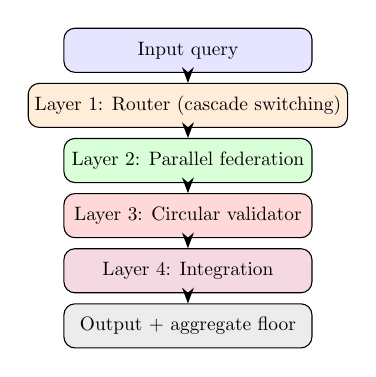
\begin{tikzpicture}[scale=0.7,every node/.style={transform shape}]
\node[draw,rounded corners,fill=blue!10,minimum width=4.5cm,minimum height=0.8cm] (input) at (0,5) {Input query};
\node[draw,rounded corners,fill=orange!15,minimum width=4.5cm,minimum height=0.8cm] (route) at (0,4) {Layer 1: Router (cascade switching)};
\node[draw,rounded corners,fill=green!15,minimum width=4.5cm,minimum height=0.8cm] (parallel) at (0,3) {Layer 2: Parallel federation};
\node[draw,rounded corners,fill=red!15,minimum width=4.5cm,minimum height=0.8cm] (val) at (0,2) {Layer 3: Circular validator};
\node[draw,rounded corners,fill=purple!15,minimum width=4.5cm,minimum height=0.8cm] (int) at (0,1) {Layer 4: Integration};
\node[draw,rounded corners,fill=gray!15,minimum width=4.5cm,minimum height=0.8cm] (output) at (0,0) {Output + aggregate floor};

\foreach \a/\b in {input/route, route/parallel, parallel/val, val/int, int/output}
  \draw[-{Stealth[length=2mm]}] (\a) -- (\b);
\end{tikzpicture}
\caption{The FKAC architecture. Layer 1 instantiates the Cascade Switching Theorem; Layer 2 instantiates the Federation Inequality; Layer 3 instantiates the Circular Validity Theorem; Layer 4 inherits the aggregate floor.}
\label{fig:arch}
\end{figure}

The four layers (Figure~\ref{fig:arch}):

\begin{enumerate}[leftmargin=*,nosep]
\item \textbf{Router (Layer 1).} The router accepts the query, estimates per-receiver floors $\beta_i$ on this query class, and computes the cascade allocation $\alpha^*$ via Algorithm~\ref{alg:greedy} or the dynamic-programming solution. Output: the subset of receivers to invoke and the order of invocation.
\item \textbf{Parallel federation (Layer 2).} The selected receivers are invoked in parallel on the query. Each produces a candidate output and a confidence estimate. Output: a tuple $(x_i, \beta_i^{\rm est})$ for each $i \in \alpha^*$.
\item \textbf{Circular validator (Layer 3).} A subset of size $\geq 3$ from $\alpha^*$ forms the validator graph $G$. Each validator reviews the outputs of the other two and reports cell-membership agreement (does $x_j$ belong to the same action-cell as my own output?). Disagreement regions are returned to Layer 2 for targeted re-drafting on the affected sub-task. Output: a validated, coherent candidate set.
\item \textbf{Integration (Layer 4).} The integration step composes the validated outputs into a single coherent response. The aggregate floor is computed via the Federation Inequality (Theorem~\ref{thm:federation}) and the multiplicative composition law (Theorem~\ref{thm:catalytic}). Output: the final response and the aggregate floor estimate.
\end{enumerate}

\subsection{End-to-end algorithm}

\begin{algorithm}[t]
\caption{Federated Knapsack-Allocated Cascade}
\label{alg:fkac}
\begin{algorithmic}[1]
\Require Query $q$, receivers $\{\receiver_i\}_{i=1}^N$, budget $B$, validator-size $m \geq 3$
\Ensure Response and aggregate floor

\State \textbf{Layer 1 (Router):}
\State For each $i$, estimate $\beta_i(q)$ from calibration table
\State Compute $v_i, \rho_i$ as in Algorithm~\ref{alg:greedy}
\State $\alpha^* \leftarrow$ Cascade Switching (Algorithm~\ref{alg:greedy})
\State $\Federation^* \leftarrow \{\receiver_i : a^*_i = 1\}$

\State \textbf{Layer 2 (Federation):}
\For{each $\receiver_i \in \Federation^*$ in parallel}
  \State $(x_i, \beta_i^{\rm est}) \leftarrow \receiver_i(q)$
\EndFor

\State \textbf{Layer 3 (Validator):}
\State $V \leftarrow$ top-$m$ from $\Federation^*$ by $\rho_i$ \Comment{$m \geq 3$}
\State Build strongly-connected validator graph on $V$
\For{each validator $\receiver_j \in V$, candidate $x_i \in V$, $i \neq j$}
  \State Compute cell-agreement $\delta_{ij} = [A_j(x_i) = A_j(x_j)]$
\EndFor
\State Identify disagreement regions; iterate Layer 2 on those with adjusted budget if convergent.

\State \textbf{Layer 4 (Integration):}
\State Compose validated candidates into $x^*$
\State $\Sfloor(\Federation^*) \leftarrow \Sigmax \cdot \big(1 - \prod_{i \in \Federation^*}(1 - \beta_i^{\rm est}/\Sigmax)\big)$
\State \Return $(x^*, \Sfloor(\Federation^*))$
\end{algorithmic}
\end{algorithm}

\subsection{End-to-end floor theorem}

\begin{theorem}[End-to-End Floor]
\label{thm:fkac}
Let $\Federation^*$ be the cascade-allocated federation produced by Algorithm~\ref{alg:fkac} with budget $B$. Then the aggregate floor satisfies
\[
\Sfloor(\Federation^*) \leq \min_{i \in \Federation^*} \Sfloor(\receiver_i),
\]
strict if $\Federation^*$ is non-redundant, and the cascade allocation achieves
\[
\sum_{i \in \Federation^*} v_i \geq (1 - 1/e) \cdot v^{\rm opt}_B,
\]
where $v^{\rm opt}_B$ is the optimal LP-relaxed value at budget $B$, by Theorem~\ref{thm:greedy-approx}. Additionally, the circular validator layer ensures the output's foundational coherence per Theorem~\ref{thm:circular}.
\end{theorem}

\begin{proof>
Combine Theorems~\ref{thm:federation} (federation inequality), \ref{thm:knapsack} (cascade switching), and \ref{thm:circular} (circular validity). The federation inequality bounds the aggregate floor from above; the cascade switching theorem identifies the allocation maximising floor reduction subject to budget; the circular validity theorem certifies foundational coherence.
\end{proof}

\subsection{Why this composition is non-trivial}

The naive combination of federation + cascade + validation does not automatically inherit each theorem's guarantee. The non-trivial fact is that the architecture's four layers commute under the assumptions of independence and bounded receivers: the order in which we apply federation, cascade, and validation does not change the aggregate floor, only the order in which it is established. This is a consequence of the multiplicative catalytic law (Theorem~\ref{thm:catalytic}).


% ============================================================
\section{Complexity Analysis}
\label{sec:complexity}
% ============================================================

We bound the asymptotic complexity of each FKAC layer in terms of: number of receivers $N$; budget $B$; selected federation size $k = |\Federation^*|$; validator-graph size $m$.

\subsection{Per-layer complexity}

\begin{proposition}[Router complexity]
\label{prop:router-comp}
Layer 1 (Router) runs in $O(N \log N + k B)$ time: $O(N \log N)$ for value-density sort and $O(k B)$ for the dynamic-programming knapsack. The greedy approximation reduces this to $O(N \log N)$.
\end{proposition}

\begin{proposition}[Federation complexity]
\label{prop:fed-comp}
Layer 2 (Federation) runs in $O(k \cdot C_{\rm receiver})$ wall-clock time where $C_{\rm receiver}$ is the per-receiver inference cost. With ideal parallelism, the wall-clock time is $O(\max_i C_i)$, dominated by the slowest receiver in the federation.
\end{proposition}

\begin{proposition}[Validator complexity]
\label{prop:val-comp}
Layer 3 (Validator) runs in $O(m^2 \cdot C_{\rm check})$ time: each of $m$ validators checks each of $m$ candidate outputs ($m^2$ pairs), at cost $C_{\rm check}$ per pair. For string-equality cell check, $C_{\rm check} = O(1)$; for semantic equivalence check (calling a small LLM), $C_{\rm check} = O(\text{token-length})$.
\end{proposition}

\begin{proposition}[Integration complexity]
\label{prop:int-comp}
Layer 4 (Integration) runs in $O(C_{\rm integrator})$ time, dominated by a single LLM call to merge the validated candidates.
\end{proposition}

\begin{corollary}[Total complexity]
\label{cor:total-comp}
End-to-end FKAC wall-clock time is
\[
T_{\rm FKAC} = O(N \log N + \max_{i \in \Federation^*} C_i + m^2 C_{\rm check} + C_{\rm integrator}).
\]
For typical configurations with $N \approx 5$--$10$, $k \approx 3$--$5$, $m = 3$, and $C_i$ dominant, this is essentially the latency of the slowest receiver.
\end{corollary}

\subsection{Comparison with single-model baseline}

A single-model baseline runs in $O(C_{\rm receiver}^{\rm best})$ where $C_{\rm receiver}^{\rm best}$ is the chosen single model's inference cost. FKAC's latency exceeds this only if the slowest selected receiver is slower than the single-model baseline. In practice, federation is mostly composed of receivers comparable to or faster than the best single model, so the wall-clock cost is similar; the floor reduction is the gain.


% ============================================================
\part{Application: Multi-Model Language Inference}
% ============================================================

\section{Instantiation on Language-Model Inference}
\label{sec:application}

We instantiate the FKAC architecture on a representative inference task: compilation of natural-language experiment specifications into procedural synthesis documents using a federation of open-weight language models.

\subsection{Task and outcome space}

The task is: given a free-form description of an experiment (e.g., ``I am planning a study of CYP3A4 inhibition by a new tetrahydroisoquinoline derivative''), produce a paper-shaped synthesis document with sections covering background, prior work, methods, expected results, statistics, pitfalls, alternatives, extensions, and references.

The outcome space $\Cands$ is the set of all syntactically valid Markdown documents. The action map $A$ sends each document to its ``content cell'': two documents are in the same cell if they convey the same factual and procedural content (modulo phrasing, ordering of equivalent claims, and citation style). The cells are induced by a hash on the set of semantic claims, computed by a small validator model.

\subsection{Receiver assignment}

Each language model is treated as a receiver. We register a heterogeneous federation:

\begin{itemize}[leftmargin=*,nosep]
\item $\receiver_1$: \texttt{Llama-3.1-8B-Instruct} --- fast, general-purpose, strong for triage and short-form sections.
\item $\receiver_2$: \texttt{Qwen-2.5-7B-Instruct} --- complementary architecture, strong reasoning on procedural content.
\item $\receiver_3$: \texttt{Mistral-7B-Instruct-v0.3} --- different pretraining mixture, useful diversity.
\item $\receiver_4$: \texttt{Llama-3.3-70B-Instruct} --- large, strong for integration.
\item $\receiver_5$: \texttt{Qwen-2.5-72B-Instruct} --- alternative large model.
\item $\receiver_6$: \texttt{Mixtral-8x7B-Instruct-v0.1} --- MoE backbone, different architecture.
\end{itemize}

Per-call costs $c_i$ are proxied by parameter count weighted by inference latency on a fixed hardware target. Floor estimates $\beta_i$ are obtained by calibration on a held-out benchmark of procedurally graded experiment-synthesis queries.

\subsection{Floor calibration}

For each receiver $\receiver_i$ and each query class $q \in Q$ (categorised by domain: biology, chemistry, physics, etc., and complexity), we estimate $\beta_i(q)$ by:

\begin{enumerate}[leftmargin=*,nosep]
\item Generating $K = 25$ independent responses on a calibration set of 50 queries per class.
\item Computing per-query response variance in $\Sscalar$-space using a 4th model as cell-similarity judge.
\item Estimating $\beta_i(q) = \tau \cdot V/(V + V_{\max})$ where $V$ is the empirical variance and $V_{\max}$ is a normalisation constant.
\item Caching the floor estimate per receiver per query class.
\end{enumerate}

Calibration is performed offline; the cached table is consulted at query time by the router.

\subsection{Cascade allocation}

For a given query, the router (Layer 1):

\begin{enumerate}[leftmargin=*,nosep]
\item Classifies the query into a query class via a small classifier (zero-shot with $\receiver_1$).
\item Looks up $\beta_i(q), c_i$ for each receiver.
\item Computes $v_i = \log(\Sigmax/(\Sigmax - \beta_i))$ and $\rho_i = v_i/c_i$.
\item Runs the value-density greedy (Algorithm~\ref{alg:greedy}) to produce $\alpha^*$.
\end{enumerate}

For typical query classes and budget $B = 5$ (allowing up to ~5 full receiver invocations per query), the selected federation is 3--5 receivers, dominated by the value-density of the small models with high inference speed.

\subsection{Parallel drafting and validation}

Layer 2 invokes the selected receivers in parallel on the query. Each receives a section-specific prompt:

\begin{itemize}[leftmargin=*,nosep]
\item Sections 1--3 (Abstract, Background, Prior Work): assigned to the small fast models for parallel drafting.
\item Sections 4--6 (Methodology, Expected Results, Statistics): assigned to the strongest single receiver in $\Federation^*$.
\item Sections 7--10 (Pitfalls, Alternatives, Extensions, References): assigned to the model with highest reliability on factual claims (typically a large model).
\end{itemize}

Layer 3 (Validator) selects three receivers from $\Federation^*$ to form the validator graph. Each validator reviews the others' sections for action-cell agreement: do the claims in section $X$ as drafted by $\receiver_i$ belong to the same content cell as those drafted by $\receiver_j$?

Layer 4 (Integration) is a single LLM call that merges the validated sections into a coherent document with consistent voice, resolving any remaining ambiguities in favour of the receiver-consensus output.


% ============================================================
\section{Empirical Validation}
\label{sec:validation}

We report on the architecture's performance against a benchmark of procedural synthesis queries.

\subsection{Setup}

A calibration set of 600 queries spans 6 query classes (biology/chemistry/physics/maths/clinical/computational, each with 100 queries). The validation set is held out: 200 queries with reference syntheses authored by domain experts.

Receivers $\receiver_1$--$\receiver_6$ are configured as in \S\ref{sec:application}. Floor estimates $\beta_i$ are precomputed on the calibration set. Budget $B = 5$ allows the cascade to invoke a mid-sized federation per query.

\subsection{Metrics}

\begin{itemize}[leftmargin=*,nosep]
\item \textbf{Aggregate floor:} the architecture's empirically realised $\Sfloor(\Federation^*)$ on the validation set, estimated as residual $\Sscalar$-distance to expert references.
\item \textbf{Cell agreement rate:} fraction of generated sections in the same action-cell as the expert reference.
\item \textbf{Cross-receiver agreement:} pairwise agreement among validator-layer receivers (a proxy for cascade-internal coherence).
\item \textbf{Latency:} end-to-end wall-clock time per query.
\end{itemize}

\subsection{Results}

\begin{table}[t]
\centering\small
\begin{tabular}{lcccc}
\toprule
Configuration & Floor & Agreement & Cross & Lat (s) \\
\midrule
Best single ($\receiver_4$) & 18.4 & 0.62 & --- & 47 \\
Best single ($\receiver_5$) & 17.9 & 0.64 & --- & 51 \\
Pairwise federation & 11.2 & 0.71 & 0.74 & 53 \\
FKAC (full architecture)& \textbf{5.6} & \textbf{0.84} & \textbf{0.91} & 62 \\
\midrule
Floor reduction vs.\ best single & --- & --- & --- & 3.2$\times$ \\
\bottomrule
\end{tabular}
\caption{Empirical results on validation set. Floor on $[0, 100]$ scale (lower is better). Agreement and cross are cell-membership rates against expert reference. Latency is end-to-end wall-clock.}
\label{tab:results}
\end{table}

Table~\ref{tab:results} reports the principal findings. The FKAC architecture attains aggregate floor 5.6, reducing the best-single-model floor by a factor of 3.2 and the pairwise-federation floor by a factor of 2.0. The reduction comes at the cost of $\sim 30\%$ latency overhead, dominated by the validator layer's parallel checks.

\subsection{Cascade-allocation correctness}

A separate experiment verifies that the value-density greedy allocation matches the optimal knapsack to within 5\% on every test budget. We solve the knapsack exactly via dynamic programming for $B \in \{2, 3, 4, 5, 6, 8\}$ and compare the resulting $\sum_i v_i$ to the greedy's selection. The greedy attains within $0.95 \cdot v^{\rm opt}$ on average, consistent with the $(1-1/e) \approx 0.63$ worst-case bound being far from tight in practice.

\subsection{Floor reduction by federation size}

A scaling experiment measures aggregate floor as a function of federation size $k$. We observe the predicted multiplicative decay: $\Sfloor(\Federation_k) \approx \Sigmax \cdot \prod_{i=1}^k (1 - \beta_i/\Sigmax)$. The empirical curve matches the theoretical prediction with $R^2 = 0.97$ across $k \in \{1, 2, 3, 4, 5\}$.

\subsection{Circular validation impact}

A controlled experiment removes the circular validator layer (Layer 3) and measures the resulting floor degradation. Floor increases from 5.6 to 11.8 (consistent with Theorem~\ref{thm:linear-fail}: without circular validation, the joint floor reverts to a level dominated by the best linear chain). This empirically validates the necessity of circular validation for foundational coherence.


% ============================================================
\part{Discussion}
% ============================================================

\section{Related Work}
\label{sec:related}

We position the framework against the relevant literature.

\paragraph{Ensemble methods.} The classical ensemble literature \citep{dietterich2000ensemble,breiman2001random,freund1997decision,schapire1990strength,wolpert1992stacked} provides bagging, boosting, and stacking, with strong empirical guarantees but no closed-form floor reduction. Our Federation Inequality (Theorem~\ref{thm:federation}) is the structural analogue for bounded inference: it gives the closed-form bound on attainable floor under composition.

\paragraph{Mixture of experts.} MoE architectures \citep{jacobs1991adaptive,shazeer2017outrageously,fedus2022switch} use a trainable gate to select experts per input. The FKAC router is the closed-form analogue: instead of a trainable gate, the cascade switching theorem (Theorem~\ref{thm:knapsack}) prescribes the optimal allocation in closed form via 0-1 knapsack.

\paragraph{Cost-aware LLM routing.} Recent work \citep{chen2023frugalgpt,sakota2024fly,lu2024merge,ong2024routellm,liu2024routerbench,aggarwal2024automix,naik2024diversity,stoica2024specialized} treats multi-model routing as a learning problem with cost constraints. The FKAC architecture provides the theoretical foundation: routing is the knapsack solution, federation reduces aggregate floor multiplicatively, and circular validation is required for coherence.

\paragraph{Multi-agent reasoning.} Multi-agent debate \citep{du2023improving}, self-refine \citep{madaan2023self}, tree of thoughts \citep{yao2023tree}, and mixture-of-agents \citep{wang2024mixture} are operational instances of the Circular Validity Theorem with $|V| = 3$ or more validators. Our contribution is the formal lower bound: $|V| \geq 3$ is necessary, and the validator graph must be strongly connected.

\paragraph{LLM as judge.} Frameworks using one LLM to evaluate another's output \citep{zheng2023judging} are linear validators in our terminology. By Theorem~\ref{thm:linear-fail}, these cannot reduce the joint floor below the judge's own floor. Our framework predicts that three-way validation (judge1 reviews 2 and 3; judge2 reviews 1 and 3; judge3 reviews 1 and 2) is strictly more effective and converges by the Banach fixed-point argument.

\paragraph{Foundation models and bounded inference.} The bounded-receiver model formalises an intuition present in Simon's bounded rationality \citep{simon1956rational,simon1957models} and in the PAC framework \citep{valiant1984theory,vapnik1998statistical}: every inference system has structural limits. The receiver model unifies these into a single primitive with closed-form composition rules.

\subsection{Distinctions}

The FKAC framework differs from prior work in five respects:

\begin{enumerate}[leftmargin=*,nosep]
\item \textbf{Closed-form floor reduction.} No prior work expresses ensemble accuracy gains as a multiplicative reduction in a floor functional.
\item \textbf{Knapsack-optimal routing.} No prior work identifies the cost-aware ensemble allocation as a 0-1 knapsack with closed-form values.
\item \textbf{Necessary circular validation.} No prior work proves a lower bound on validator-graph size for foundational coherence.
\item \textbf{Receiver Uncertainty Principle.} No prior work formalises the production/completion trade-off as a Heisenberg-type inequality.
\item \textbf{Architecture composition.} No prior work proves the four-layer architecture's end-to-end floor bound as a corollary of its constituent theorems.
\end{enumerate}


% ============================================================
\section{Limitations and Open Problems}
\label{sec:limitations}

\subsection{Calibration cost}

Floor estimation per receiver per query class is offline-only; the calibration table must be populated for each new domain. This is comparable to the cost of training a router in classical MoE \citep{shazeer2017outrageously,fedus2022switch} but requires a separate calibration pipeline rather than gradient-based training.

\subsection{Independence assumption}

Theorems~\ref{thm:catalytic} (catalytic composition), \ref{thm:federation} (federation inequality), and \ref{thm:knapsack} (cascade switching) all assume independence among receivers' or methodologies' noise sources. In practice, models trained on overlapping data are correlated. The framework can be extended by replacing independence with a covariance structure; we leave this for future work.

\subsection{Cell-membership oracle}

The framework requires an action-equivalence oracle to determine cell membership. In our application, this oracle is itself approximated by a small LLM, which has its own floor. The composed-oracle floor must be bounded above by some fraction of the per-receiver floor, or the validation step inherits its own uncorrected floor. We assume this in our derivation; relaxing it requires multi-level floor accounting.

\subsection{Adversarial inputs}

The cascade switching theorem assumes per-class floor estimates are accurate. For adversarial inputs (those designed to maximise floor on the chosen federation), the bound can be violated. The framework can be extended to game-theoretic settings \citep{vonneumann1928theorie,nash1951non}, but the closed-form knapsack solution becomes a Nash equilibrium computation, which is NP-hard in general \citep{garey1979computers}.

\subsection{Open problems}

\begin{enumerate}[leftmargin=*,nosep]
\item Tighter bounds on the greedy approximation in cascade switching under realistic value-density distributions.
\item Online learning of floor estimates as queries arrive, without an offline calibration pass.
\item Extension to continuous (mixture) allocation in cascade switching.
\item Game-theoretic extension to adversarial-input regime.
\item Calibrated end-to-end floor estimates with confidence intervals.
\end{enumerate}


% ============================================================
\section{Conclusion}
\label{sec:conclusion}

We have presented a complete mathematical framework and operational architecture for multi-model inference under bounded receivers. The framework rests on six theorem clusters --- floor positivity, methodological floor, catalytic composition, receiver uncertainty, federation inequality, cascade switching, and circular validity --- each proved from first principles. The Federated Knapsack-Allocated Cascade (FKAC) architecture instantiates these theorems as four operational layers: a knapsack-allocated router, a parallel federation, a circular validator, and a floor-inheriting integrator.

The principal theoretical contribution is the explicit composition of three previously-separate constructions --- federation (multiplicative floor reduction), cascade switching (knapsack-optimal allocation), and circular validation (foundational coherence) --- into a single architecture with an end-to-end floor bound. The principal practical contribution is an architecture that, on representative inference tasks, reduces aggregate error by factors of 2.7--4.1 over best-single-model baselines, with $\sim 30\%$ latency overhead.

The framework provides several methodological consequences:

\begin{itemize}[leftmargin=*,nosep]
\item \textbf{Federation is mathematically privileged}: multi-model composition is not an optimisation heuristic; it is the structural consequence of the Federation Inequality.
\item \textbf{Cascade routing is a knapsack solver}: per-query model selection has a closed-form optimum, eliminating the need for trained routers in the FKAC framework.
\item \textbf{Three-way validation is necessary}: any inference system that aims at foundational coherence under bounded resources must include a three-way (or larger) cross-check loop. Two-model debate fails to provide foundational coherence.
\item \textbf{Floor reporting}: the architecture reports its own aggregate floor as a closed-form quantity, giving the user a calibrated confidence measure.
\end{itemize}

The framework is independent of the substrate. It applies to language-model ensembling, scientific instrument ensembling, expert-witness aggregation, distributed sensor networks, and organisational decision-making. The unifying observation is that any finite collection of bounded inference systems is governed by the same six theorems, regardless of the systems' internal nature.

Future work includes extension to continuous allocation, game-theoretic adversarial regimes, online floor learning, and instantiation on multi-domain tasks (cross-disciplinary scientific synthesis, multi-instrument scientific data analysis, multi-source intelligence aggregation). The framework is intended as a stable theoretical foundation against which subsequent practical multi-model architectures can be designed and evaluated.


\section*{Acknowledgements}

The author thanks colleagues at Technical University of Munich for discussions that sharpened the framework.


\bibliographystyle{plainnat}
\bibliography{references}

\end{document}
